\section{Matched optimization study}\label{sec:optimization}
This section tests whether adjoint-driven optimization shortens the time
needed to reach a common validated ripple target. The protocol and all of
its amendments were fixed in the
\href{https://github.com/rjwalters/geode-fem/issues/1185}{preregistration}
before any main-run outcome was observed. One later deviation, in how the
final refinement was run, was adopted after the main runs had finished and
is described with the refinement in Section~\ref{sec:exp2-refinement}; it
changes no selection rule, check or target. The finite-difference ablation
of Section~\ref{sec:exp2-fd} was added after the main outcomes were known
and is not part of the preregistered study.

\subsection{Protocol}
\paragraph{Methods.}
Five methods form an optimizer-by-resolution comparison plus one
surrogate (Table~\ref{tab:methods}). A and E are SLSQP
\citep{kraft1988} using the field adjoints of Section~\ref{sec:gradients},
safeguarded so that a refused request restores the last admissible point
and restarts the solver; B and D are COBYQA \citep{ragonneau2022} with $2n+1$ interpolation points
and unit-box trust radii $0.1$ to $10^{-6}$, where $n$ is the number of free
parameters. Both run through SciPy 1.18.1 \citep{virtanen2020scipy}. C is
an empirical trust-region method on four cubic radial-basis interpolants
of the L1 training outputs (the three per-current standard deviations and
the full-current mean), refitted after every evaluation from an $n+1$-point
initial design; Appendix~\ref{sec:settings} gives its radii, acceptance
and update rules and the other settings. A/B and E/D vary the optimizer at fixed training resolution,
and A/E and B/D vary resolution at fixed optimizer. The optimizer contrast
includes differences in search strategy, so it does not isolate gradient
access as the only causal difference. Training uses order-45 coupling torque
on 20 angles at current fractions $0$, $\tfrac12$ and $1$ of the fixed peak
current $9.6777\,\mathrm{A}$. L0 and L1 differ only in spatial resolution,
and neither is fitted or corrected against validation. Time to a fixed
target, with unattained targets kept as censored, follows the data- and performance-profile
practice for benchmarking optimization solvers \citep{more2009benchmarking,dolan2002benchmarking}.
The preregistration also named a fixed group-1 current-density rule as a
labelled control. It was not run in this study, which uses the fixed
physical current throughout; Section~\ref{sec:gradients} reports that
rule's effect on sensitivities.

\begin{table}[H]\centering\small
\caption{Methods. D and E solve the coarse nonlinear field equations; they
are neither fitted magnetic circuits nor reduced-basis models.}
\label{tab:methods}
\begin{tabular}{lll}\toprule
Method & Optimizer or search model & Training mesh\\\midrule
A & Safeguarded SLSQP, field adjoints & L1\\
B & COBYQA, forward evaluations & L1\\
C & Empirical cubic-RBF trust region & L1\\
D & COBYQA, forward evaluations & L0\\
E & Safeguarded SLSQP, field adjoints & L0\\\bottomrule
\end{tabular}
\end{table}

\paragraph{Design spaces and constraints.}
Space A has eight free geometric lengths: MAG, MH, MW, SW1--SW4 and Sr1
(Appendix~\ref{sec:parameters}), that is, the rotor iron depth, magnet
height and width, four stator tooth and slot dimensions, and the slot-bottom
fillet radius. Space B adds ten grouped offsets acting on 55 surface control
points. Stack length, radial scale, stator outer diameter and operating
angle are fixed, so the saved Opt120 design lies outside both spaces. The
two spaces also use different discrete mesh-motion maps, so their contrast
does not isolate the ten added offsets.
Each training model $r\in\{\mathrm{L0},\mathrm{L1}\}$ minimizes
$F_r=\sum_c\sigma_{r,c}^2$ over the three training currents, subject to
$\mu_{r,1}\geq1.0025\,\mu_{r,1}(\theta_0)$ for its own full-current mean and to
normalized construction margins $c_i-0.05\geq0$. Unbuildable or
mesh-infeasible candidates are refused: SLSQP restores toward the last
admissible point and restarts, COBYQA receives a NaN barrier, and C skips
the point. A moved mesh with an inverted triangle or a minimum angle below
$5^\circ$ is repaired by up to four charged remeshing attempts. Because
refinement cannot remove a limiting geometric corner, the $5^\circ$ policy
also acts as an implicit geometric constraint. Space B's slot-opening
channel wall is not guarded and can become very thin at extreme offsets;
that risk is handled by repair and refusal, not by a wall-thickness
constraint.

\paragraph{Training gradients.}
Section~\ref{sec:gradients} verifies a different, scalar parameter set; the
gradients that A and E use were checked separately. In both spaces, the L1
training objective $F$ and full-current mean were compared with central
differences at $\theta_0$ and at an interior point, along a fixed
box-scaled direction and for three (space A) or four (space B) components,
including the offsets CPR1 and CPS1. With Newton tolerance $10^{-12}$, the
directional relative errors at $h=10^{-4}$ are $1.5\times10^{-8}$ to
$2.8\times10^{-7}$ for $F$ and $2.4\times10^{-9}$ to $4.7\times10^{-9}$ for
the mean, and the component errors at $h=10^{-6}$ are at most
$2.8\times10^{-6}$. The directional error falls by 72 to 156 times from
$h=10^{-3}$ to $10^{-4}$, as truncation error should. The evaluator's own
gradient replies at the study's training tolerance of $10^{-8}$ agree at
the interior point within $3.1\times10^{-6}$ directionally; the largest
component error, $4.3\times10^{-5}$, belongs to the small Sr1 derivative.
At $\theta_0$, space B's offsets sit on their bounds, so the central
stencils there step outside the design box. The records are pinned with the
optimization harness (Code and data availability).

\paragraph{Common validation and credit.}
Every method is judged on the same order-93, L2, 20-angle validation model.
Its initial-design anchor is $F_0=9.6034\times10^{-3}\,\mathrm{N^2\,m^2}$ with
full-current mean $\mu_0=1.44084\,\Nm$. The targets are $T_{50}=0.5F_0$,
$T_{90}=0.1F_0$ and $T_{99}=0.01F_0$. A validated design attains a target
only if
\begin{equation}
 F_{\mathrm{val}}+\delta F\leq T,\qquad
 \delta F=\max\{0.10F_{\mathrm{val}},\,2.5\times10^{-7}\,\mathrm{N^2\,m^2}\},
\end{equation}
its validated full-current mean is at least $1.0025\,\mu_0$, its
construction margins and mesh checks pass, and its validation completes
within budget. The allowance $\delta F$ is an empirical margin, not a bound
on continuum error. Optimizer success flags confer no credit. Changed
incumbents are validated as they appear, after the initial interpolation
set for B, C and D.

\paragraph{Budget and timing.}
Cost is wall time, in units of the median cold validation forward measured
on the same host at the same concurrency. Each run receives 120 units,
with a 60-unit checkpoint that counts only validations completed by then.
The charge covers evaluator start-up, geometry checks, mesh motion and
repair, training solves, adjoints, optimizer overhead, surrogate fitting
and validation; nothing is subtracted as overhead. L0 receives no discount.

\paragraph{Starts and execution.}
Each space uses $\theta_0$ and four Latin-hypercube starts (seeds 1--4),
with the scalar coordinates matched across spaces. A start was eligible
only if it was buildable and admissible, and its moved reference mesh met
the mesh policy without repair, in both spaces at L0 and L1. The starts
therefore favor moderate deformations and are not uniform samples of the
design box. All starts were frozen before any main outcome. Every method
runs from every start twice, giving 100 runs. Within a start, repeat 1
rotates the method order and repeat 2 reverses it.

The session ran on one AWS c7a.4xlarge host (x86-64; NumPy 2.5.4 and
SciPy 1.18.1 with OpenBLAS) with 15 concurrent single-threaded processes.
Before calibration, the host recomputed the initial-design validation
waveforms in both spaces. $F_0$ agreed with the canonical anchor to
$2.4\times10^{-13}$ relative, within the preregistered $10^{-9}$ tolerance,
and the two spaces agreed bit for bit. The calibrated unit was
$70.94\,\mathrm{s}$, the median of 45 concurrent cold validations. All 100
runs completed in one session with no recovery, deferral or contamination:
the one-minute load average peaked at 21.1, below the contamination
threshold of $1.5N=22.5$. The in-run cost totals 109~CPU-hours. Of the
100 runs, 38 stopped on reaching $T_{99}$, 46 on optimizer convergence and
13 at the budget. The other three are SLSQP runs (A) in space A whose
solver stopped without converging: both repeats from LHS~2, after about 43
units, and repeat~1 from LHS~3, after 119 units.

\subsection{Results}
\paragraph{Repeats.}
The two repeats of each run follow the same optimization path. In all 50
pairs, the sequences of validated objectives agree exactly up to the
shorter run's length, and they differ in length only when the budget or a
solver stop cuts one repeat earlier. The repeats therefore measure timing
noise, not independent outcomes, and the comparison is a paired case study
over five starts. Over the 111 target crossings attained in both repeats,
the time differs by a median of 2.1\% and at most 12.4\% relative to
repeat~1. Repeat-1 times are reported below.

\paragraph{Attained quality.}
Figure~\ref{fig:exp2-quality} shows the best credited value of
$(F+\delta F)/F_0$ for every start, method and space (repeat~1).
In space A, no run goes below $F/F_0=0.043$ and none reaches $T_{99}$.
The best designs of A, B, D and E all reach $0.043F_0$, and C's reaches
$0.049F_0$; in Fig.~\ref{fig:exp2-quality}, which includes the allowance,
the A, B, D and E level appears near $0.048$ (C's near $0.054$). All five lie within 0.17\% above the
full-current mean floor, so the mean constraint is active there: the level
shared by A, B, D and E is the constrained optimum they found in the
eight-parameter space,
not a property of any one method. In space A the start mattered more than
the method. From LHS~4, A and B stop near $0.09F_0$, D reaches $0.044F_0$,
and C and E never produce a credited validation, in either repeat. In
space B, each method's best design reaches $0.004$--$0.009F_0$, and every
method except C reaches $T_{99}$ from at least four of five starts.

\begin{figure}[t]\centering
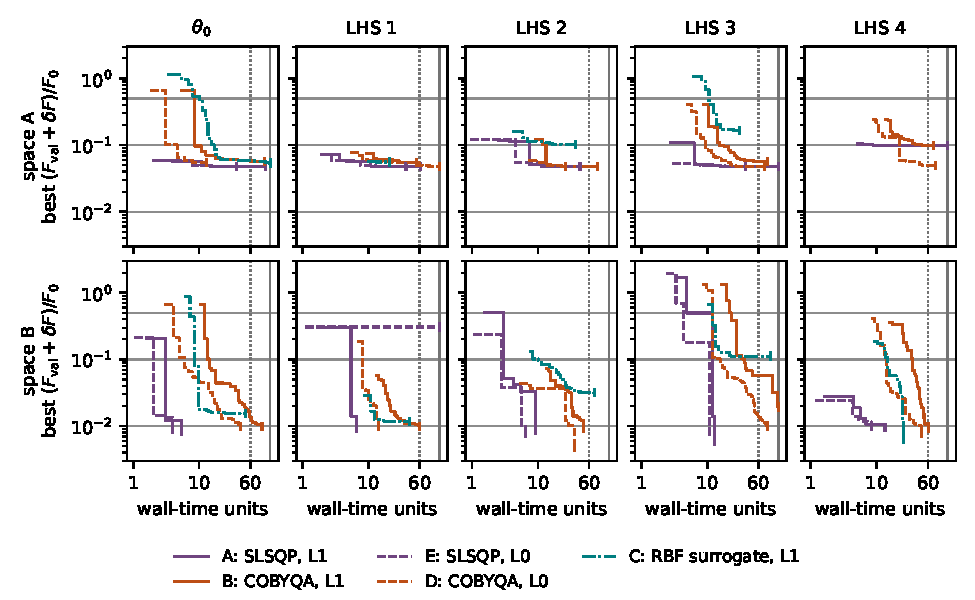
\includegraphics[width=\linewidth]{figures/exp2-quality.pdf}
\caption{Best credited $(F_{\mathrm{val}}+\delta F)/F_0$ versus charged wall
time, repeat~1, at common L2/order-93/20-angle validation. Grey lines mark
$T_{50}$, $T_{90}$ and $T_{99}$; the dotted and solid vertical lines mark
the 60-unit checkpoint and the 120-unit budget. The time axis is
logarithmic. Each curve ends at the run's actual stop (tick). A missing curve
means the run had no credited validation.}
\label{fig:exp2-quality}
\end{figure}

\paragraph{Time to target.}
Figure~\ref{fig:exp2-time} gives the charged time to each target, per
start, and Table~\ref{tab:exp2-time} in Appendix~\ref{sec:exp2-times} lists
the values. In repeat~1, only three crossings occur
after the 60-unit checkpoint, all at $T_{99}$ in space B: two by B and one
by D.

Table~\ref{tab:exp2-ratios} (Appendix~\ref{sec:exp2-times}) gives paired time ratios. A ratio is formed
only when both methods attain the target from that start; no finite ratio
is derived from a censored cell. Wherever both reach a target from the
same start, gradient-based SLSQP gets there sooner than COBYQA at the same
training resolution. At L1 (B/A), the geometric-mean ratio is 3.10--3.25 in
space A and 5.06--7.79 in space B. At L0 (D/E), it is 2.45--2.75 and
3.14--7.20.
All 45 finite optimizer-contrast pairs (by space, target and start) favor
SLSQP, with ratios from 1.46 to 21.5. The coarse mesh shortens the time by
a smaller factor: the geometric-mean E/A ratio is 0.62--0.79 and D/B is
0.45--0.56. As charged, A is faster than D, the inexpensive derivative-free
physical competitor, by a geometric mean of 1.68--1.83 in space A and
2.25--4.32 in space B. This contrast changes both factors; one of its 25
pairs is a near tie (0.99, space-A LHS~2 at $T_{90}$: D is 0.75\% faster,
within the timing noise between repeats), and in space A most of the
contrast comes from validation charges (next paragraph). We conjecture that part of the larger
space-B ratios comes from COBYQA's initial interpolation set, which costs
$2n+1=37$ training evaluations before its first model step there, against
17 in space A.

\paragraph{Validation charges.}
Validating every new incumbent makes validation the largest single
charge (Table~\ref{tab:exp2-validation}). One validation costs a median of
0.87 units over the 3,350 completed validations (range 0.55--1.10), and
validation takes 53\% of all charged time, 2--90\% per run. SLSQP crosses
a target after few validations, but most of its time to a target is
validation; COBYQA at L1 (B) needs more validations, which are a smaller
part of its time. Excluding the validation charges up to each crossing, the
same-resolution geometric means rise to 5.41--5.66 (B/A) and 5.55--5.56
(D/E) in space A, and to 8.84--13.58 and 7.92--15.27 in space B, so the
ratios as charged are conservative for the optimizer contrast. The coarse
mesh cuts the remaining time more, by geometric means of 0.19--0.27 (E/A)
and 0.20--0.23 (D/B), but it does not make validation cheaper, which is why
its overall saving is only 1.3--2.2 times. The space-A contrast between A
and D does not survive this decomposition: excluding validation, its
geometric mean is 1.15--1.16, and two of its ten space-A pairs favor D
(0.97 and 0.54). In space A, A's lead over D therefore reflects mainly how
many validated incumbents each method needs before crossing under the
validate-every-incumbent rule (medians of two and six). In space B the
non-validation D/A mean remains 1.92--3.19.

\begin{table}[tbp]\centering\small
\caption{Validation charges, repeat~1. ``To crossing'' counts the
validations up to and including the first attaining one, and ``share''
gives the fraction of the time to that target charged to validation, as
medians (ranges) over the method's attained targets and starts. ``Run''
gives the range over starts of the fraction of the whole run's charged time
spent in validation.}
\label{tab:exp2-validation}\begin{tabular}{lllllll}\toprule
 & \multicolumn{3}{c}{Space A} & \multicolumn{3}{c}{Space B}\\\cmidrule(lr){2-4}\cmidrule(lr){5-7}
Method & To crossing & Share & Run & To crossing & Share & Run\\\midrule
A & 2 (2--7) & 0.65 (0.65--0.71) & 0.45--0.71 & 3 (1--10) & 0.61 (0.58--0.68) & 0.65--0.68\\
B & 5 (2--25) & 0.46 (0.22--0.53) & 0.24--0.34 & 8 (2--36) & 0.34 (0.15--0.45) & 0.35--0.49\\
C & 6.5 (2--10) & 0.53 (0.42--0.64) & 0.02--0.63 & 4 (2--17) & 0.40 (0.25--0.56) & 0.50--0.61\\
D & 6 (2--20) & 0.81 (0.60--0.84) & 0.41--0.64 & 9 (2--70) & 0.71 (0.46--0.77) & 0.73--0.77\\
E & 2 (1--5) & 0.90 (0.87--0.92) & 0.82--0.90 & 3 (1--11) & 0.88 (0.83--0.90) & 0.87--0.90\\
\bottomrule\end{tabular}

\end{table}

The speed of E has a reliability cost. E never produces a credited
validation from space-A LHS~4. From space-B LHS~1 it reaches $T_{50}$ but
then stalls at $0.28F_0$, missing $T_{90}$ and $T_{99}$. In four
start--target cells, D reaches a target that E misses. A, by contrast,
reaches every target that any method reaches, from every start. C attains
$T_{99}$ only once in space B and reaches $T_{90}$ from two of five
space-A starts.

\begin{figure}[t]\centering
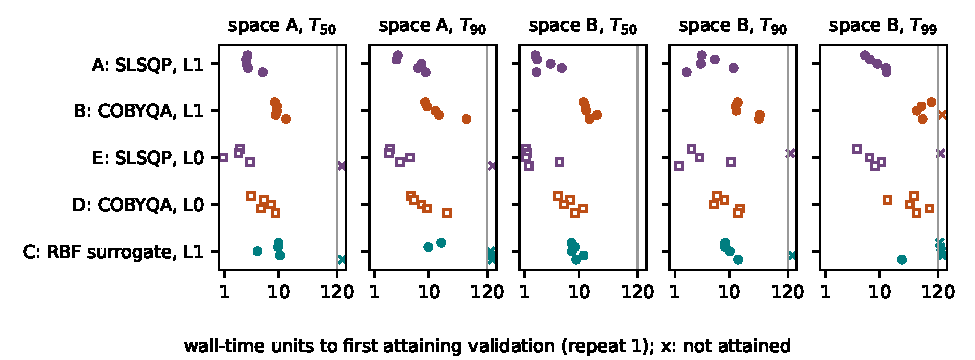
\includegraphics[width=\linewidth]{figures/exp2-time-to-target.pdf}
\caption{Charged wall time to the first attaining validation, repeat~1, one
marker per start, for every target attained by some run. Filled markers:
L1 training; open markers: L0 training; crosses: not attained within 120
units.}
\label{fig:exp2-time}
\end{figure}

\paragraph{Final refinement.}\label{sec:exp2-refinement}
The preregistered selection takes, for each method and space, the
lowest-$F_{\mathrm{val}}$ feasible design over both repeats, and the
earliest repeat-1 crossing of each attained target. With $\theta_0$ in
each space and identical designs merged, this gives 33 designs. Each
received the six registered checks: the primary L2 validation, L3, a
40-angle grid, Newton tolerance $10^{-12}$, an independently solved grid
shifted by $0.5^\circ$, and held-out currents $0.25$ and $0.75$. The 15
designs with zero stator offsets also received the conforming outer-band
Arkkio check on fresh meshes. All 213 checks completed
(Table~\ref{tab:exp2-refinement} in Appendix~\ref{sec:exp2-times}). These checks qualify the selected
designs only; they do not check each of the study's 111 repeat-1
target crossings.

The registered pipeline begins by capturing the closed study on its
original host, a step that could not be completed after that host had been
restarted. The refinement instead used a copy of the study outputs whose
integrity is established by a SHA-256 inventory of every output file, taken
when the session finished, and independently timestamped; the timestamps
establish that the inventory existed by 2026-10-20 03:50~UTC. It ran on a different host (Apple M3 Ultra,
macOS arm64). For the 16 selected designs validated on the moved reference
mesh, the primary check reproduces the study's $F_{\mathrm{val}}$ to below
$2.2\times10^{-12}$ relative. The other 15 candidates needed a fresh mesh,
which Gmsh triangulates differently on the two platforms; their $F$
differs by at most $1.7\times10^{-3}$ relative. The remaining two designs
are $\theta_0$ in each space, which reproduces $F_0$. The fresh-mesh
differences measure the sensitivity of $F$ to remeshing and are far below
the 10\% allowance $\delta F$.

Spatial refinement is the largest change. Over all 33 designs, L3 moves
$F$ by $-4.0\%$ to $+6.3\%$. Over the 25 target crossings alone, the range
is $-4.0\%$ to $+1.1\%$. The largest increase belongs to the overall best
design, D's in space B, whose $F$ rises from $0.0044F_0$ to $0.0047F_0$.
Angular and nonlinear effects are small: the 40-angle and shifted grids
change $F$ by at most $0.11\%$, and the tighter Newton tolerance by less
than $1.1\times10^{-5}$ relative. The conforming estimator gives $1.1\%$ to
$4.4\%$ more ripple than the order-93 coupling on the space-A designs, and
$2.0$--$2.1\%$ more at $\theta_0$. All 25 target crossings still satisfy
their target, allowance included, at L3; the smallest remaining margin is
1.2\% of the target. Every candidate also satisfies the full-current mean
floor in the primary, L3, 40-angle, tight and shifted checks, the closest
by 0.012\%. The refinement therefore confirms the selected crossings and
leaves the time-to-target comparison unchanged.

The held-out currents test the ripple reduction outside the three training
currents. We compare each design's objective at currents $0.25$ and $0.75$,
relative to $\theta_0$'s at the same currents, with its relative objective
at the training currents. Across the candidates, the held-out ratio is 0.65
to 1.73 times the training-current ratio; values above one mean a smaller
reduction at the held-out currents. For the five best space-A designs it
is 1.07--1.09. In space B, four of the five best designs keep less of
their reduction: their remaining objective fraction at the held-out currents
is 1.23--1.73 times that at the training currents, while for B's best
design it is 0.89. D's best design has $0.0044F_0$ at the training currents but
$0.0076$ of $\theta_0$'s value at the held-out currents. Part of the extra
reduction from space B's added freedom is therefore specific to the three
training currents.

The training model also reads lower than validation. At $\theta_0$, the
order-45 training objective is 0.887 (L1) and 0.894 (L0) of $F_0$. At the
31 selected designs, the ratio of training to validation objective lies
between 0.57 and 1.19 times its $\theta_0$ value. The lowest values belong
to space-B designs near $T_{99}$: E's and A's $T_{99}$ crossings (0.57 and
0.71) and D's best design (0.65); the best space-B designs of B and C are at
0.99 and 1.19. Large reductions therefore often, but not always, come with a
training objective that underestimates validation more than at $\theta_0$.
This is consistent with the cancellation conjecture of
Section~\ref{sec:opt120} but does not establish it.

\subsection{Post-hoc ablation: finite-difference SLSQP}\label{sec:exp2-fd}
The contrasts above vary the optimizer together with gradient access. This
ablation varies gradient access alone. It was added after the main
outcomes were known, so it is post hoc and not part of the preregistered
study; its protocol was frozen in a
\href{https://github.com/rjwalters/geode-fem/issues/1218}{separate public protocol}
before any of its runs.

\paragraph{Protocol.}
Method F is the safeguarded SLSQP of A with identical bounds, constraints,
restoration, validation policy, targets, mean floor and stopping rules.
Only the gradients of the objective and of the mean constraint change: they
are forward differences of training values with a step of $10^{-6}$ in each
component's unit, reusing the base value, so one gradient costs $n+1$
training forwards ($n=8$ in space A and 18 in space B). A component whose
forward step is inadmissible or would remesh uses the backward step; if
both fail, the gradient is refused as it would be for A. Every
difference solve is charged to the run. The geometry-constraint Jacobians
remain analytic, as for A. To make the comparison within one session, A is
rerun unchanged in the same session as A$'$: both methods run from the five
starts above, in both spaces, with two repeats and rotated method order,
giving 40 runs of 120 units on the L1 training model. The primary estimand
is, per start, the repeat-1 ratio F/A$'$ of time to $T_{90}$ in space A and
to $T_{99}$ in space B; a censored cell gives no finite ratio. The
representative and earliest crossings of F receive the six refinement
checks above.

\paragraph{Results.}
Per-start F/A$'$ time ratios and their geometric means: [PENDING exp2b-fd-slsqp].
Hit fractions and censoring of F and A$'$: [PENDING exp2b-fd-slsqp].
Consistency of A$'$ with the main-study A and repeat-2 reproducibility:
[PENDING exp2b-fd-slsqp].
Final refinement of F's selected designs: [PENDING exp2b-fd-slsqp].

\paragraph{Gradient credit.}
[PENDING exp2b-fd-slsqp]
